\clearpage
\subsubsection{Union} % (fold)
\label{ssub:union}

A Union (Variant Record in Pascal) allows you to declare a type where the values may be one of a range of alternative types. In effect, you can declare a type where the value may be one of a number of different types. This is useful if you want to store different types of values at a location in your program.

A Union often works best by accompanying it with a \textbf{tag} value. This value then records the kind of data currently being stored at the location in memory. A good option is to use an \nameref{ssub:enum} for the tag's type, giving you a range of value, that describe the range of types stored.

\begin{figure}[h]
   \centering
   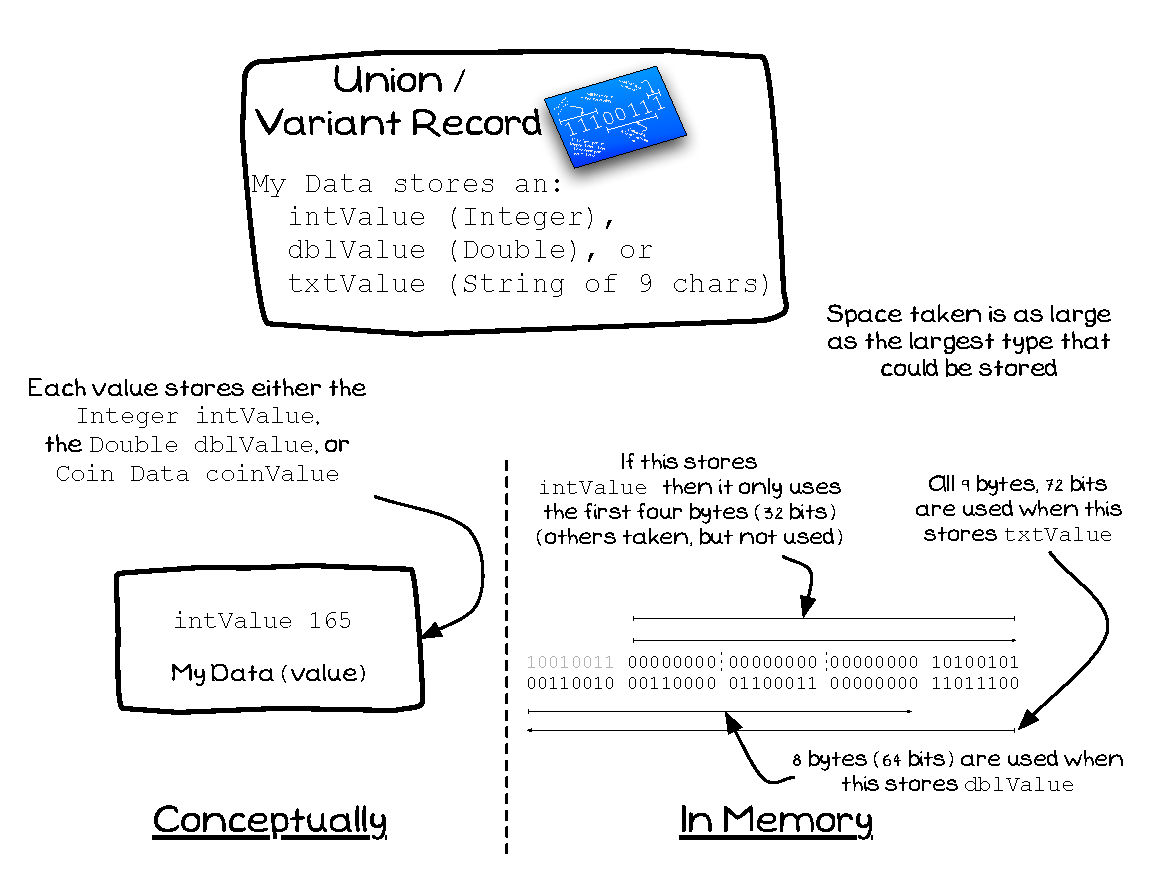
\includegraphics[width=\textwidth]{./topics/type-decl/diagrams/Union} 
   \caption{A Union is one type that can store one of a range of other types}
   \label{fig:type-decl-union}
\end{figure}

\mynote{
\begin{itemize}
  \item A Union is a kind of \texttt{artefact} that you can declare. 
  \item The Union allows you to use one location in memory to store one of a number of types of value.
  \item At any one time this data can be used to store \textbf{one} of these values.
  \item It is the developers responsibility to ensure they access the right kind of value when it is being used.
  \item A \textbf{tag} value can be used to store a marker that indicates the type of data being stored in the union.
  \item The \textbf{size} of a union is the size of its \emph{largest} option. For example a union of a \texttt{Character} (1 byte), a \texttt{Integer} (4 bytes), and a \texttt{Double} (4 bytes) is 4 bytes, the size of the largest kind of value it needs to store.
\end{itemize}
}

% subsubsection union (end)